\documentclass[titlepage,a4paper,oneside]{article}
\usepackage[utf8]{inputenc}
\usepackage{amsmath}
\usepackage{mathabx}
\usepackage{graphicx}
\usepackage{minted}
\usepackage{booktabs}
\usepackage[english,spanish,es-noindentfirst,es-nosectiondot,es-nolists,
es-noshorthands,es-lcroman,es-tabla]{babel}
\usepackage{lmodern}             % Use Latin Modern fonts
\usepackage[T1]{fontenc}         % Better output when a diacritic/accent is used
\usepackage[utf8]{inputenc}      % Allows to input accented characters
\usepackage{textcomp}            % Avoid conflicts with siunitx and microtype
\usepackage{microtype}           % Improves justification and typography
\usepackage[svgnames]{xcolor}    % Svgnames option loads navy (blue) colour
\usepackage[hidelinks,urlcolor=blue]{hyperref}
\hypersetup{colorlinks=true, allcolors=Navy, pdfstartview={XYZ null null 1}}
\newtheorem{lemma}{Lema}
\usepackage[width=14cm,left=3.5cm,marginparwidth=3cm,marginparsep=0.35cm,
height=21cm,top=3.7cm,headsep=1cm, headheight=1.6cm,footskip=1.2cm]{geometry}
\usepackage{csquotes}
\usepackage{biblatex}
\addbibresource{informe.bib}
\usepackage[pdf]{graphviz}


\begin{document}

\begin{titlepage}
\title{
	75.74 \-- Distribuidos I \-- TP2\\
    \large Facultad de Ingeniería\\
	Universidad de Buenos Aires
}
\author{
	Mermet, Ignacio Javier\\
	\texttt{98153}
}
\date{Mayo 2022}

\maketitle

\end{titlepage}

\tableofcontents

\newpage

\section{Sobre la entrega}
El código de la entrega se puede encontrar en \href{https://github.com/CrossNox/7574-TP2}{GitHub}.

\section{Estructura del proyecto}
El proyecto fue desarrollado en \texttt{python}\cite{Python} y empaquetado con \texttt{poetry}\cite{PythonPoetry}. Tiene dos CLIs asociadas:

\begin{itemize}
	\item \texttt{rma}:
	\item \texttt{rma\_client}:
\end{itemize}

En la carpeta \texttt{docker} se encuentra disponibles el \texttt{Dockerfile} asociado al paquete.

\section{Instalación y ejecución}
Referirse al archivo \texttt{README.md} provisto en el repositorio para ver las instrucciones de instalación.

\section{DAG}
El diseño del DAG se hizo en base a la premisa de filtrar la mayor cantidad de datos lo antes posible. Del mismo, modo, evitar reprocesamiento que tenga la misma salida.

Los nodos se plantearon no en base a unidades de ejecución que reciben el mismo input, sino en unidades que conceptualmente hacen el mismo tipo de tareas. Por ejemplo, filtros o transformaciones.

\begin{figure}[H]
\centering
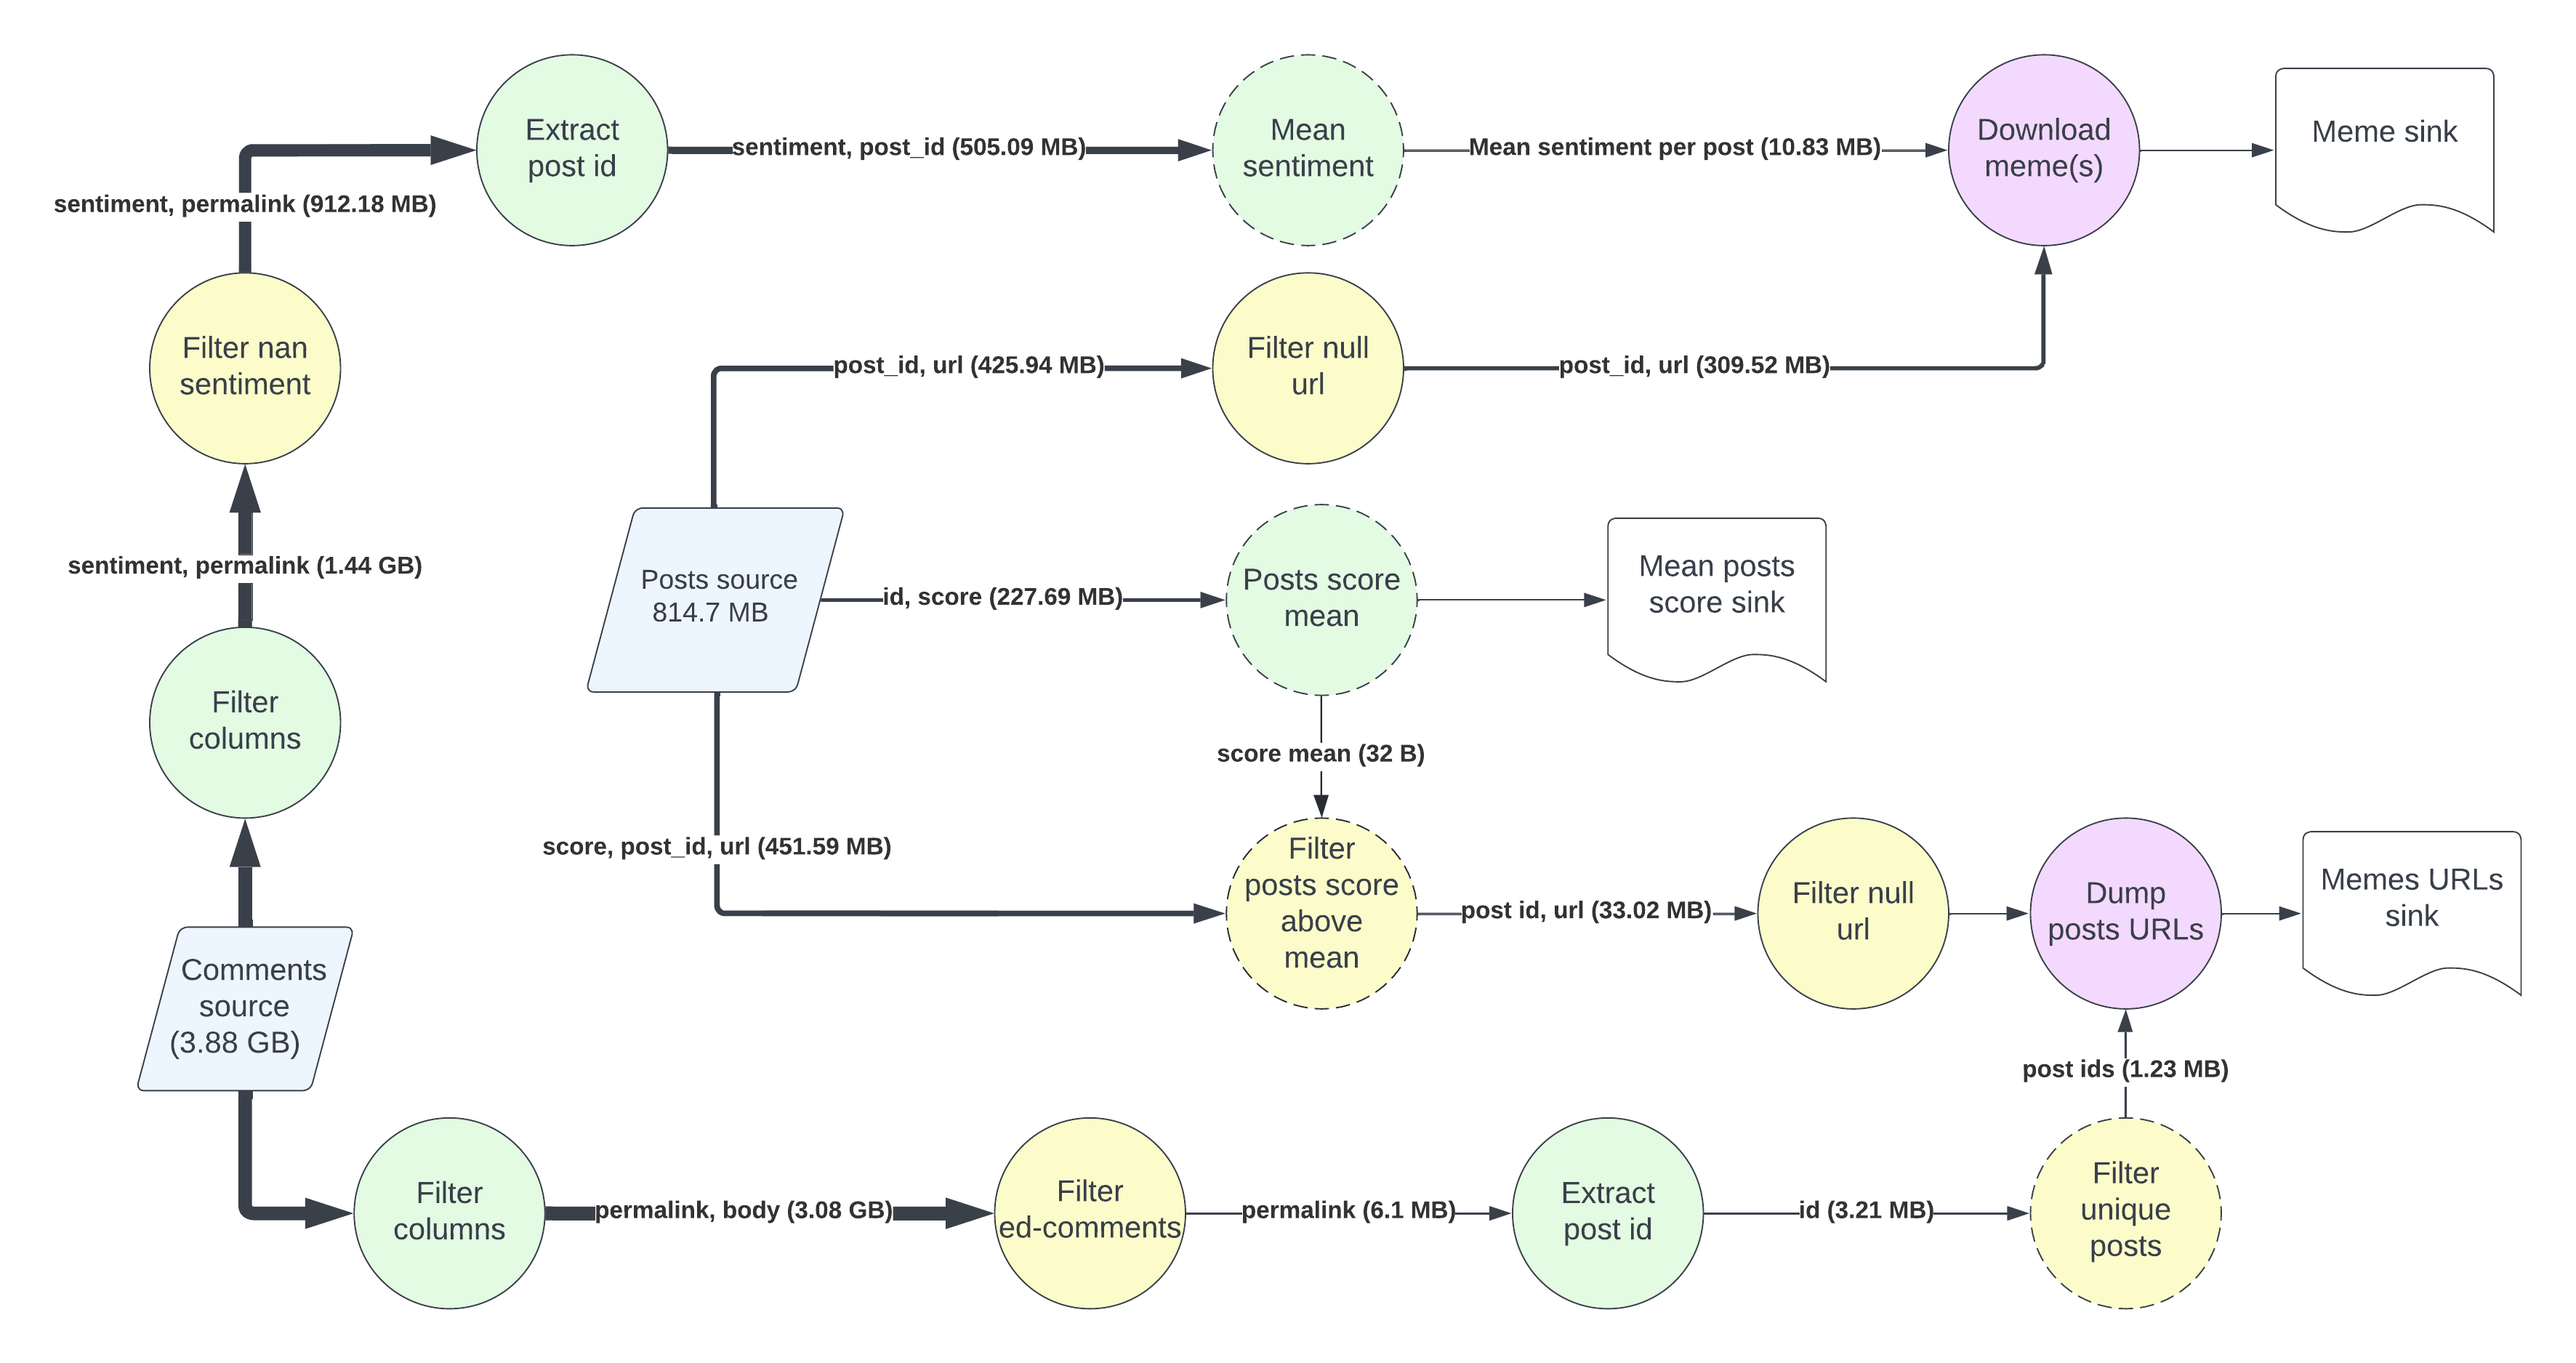
\includegraphics[width=\textwidth]{images/DAG.png}
\caption{DAG diseñado}
\end{figure}

\textbf{Nota} sobre los colores.
\begin{itemize}
	\item Rosa: \texttt{Join}
	\item Verde: \texttt{Transformation}
	\item Azul: \texttt{Source}
	\item Amarillo: \texttt{Filter}
\end{itemize}

Las líneas punteadas significan que los resultados de esos nodos no pueden ser obtenidos hasta haber procesado la totalidad de los datos entrantes. Los números entre paréntesis son valores aproximados del tamaño de la salida de cada nodo. No sería adecuado pensarlos en valores absolutos, sino más bien, son ilustrativos en valor relativo. Estos valores se obtuvieron con \texttt{pandas}, viendo el tamaño en memoria del dataframe resultante de la operación (con los parámetros \texttt{memory\_usage=``deep''} y \texttt{index=False}).

\subsection{DAG Generado desde RMA}
\begin{figure}[H]
\centering
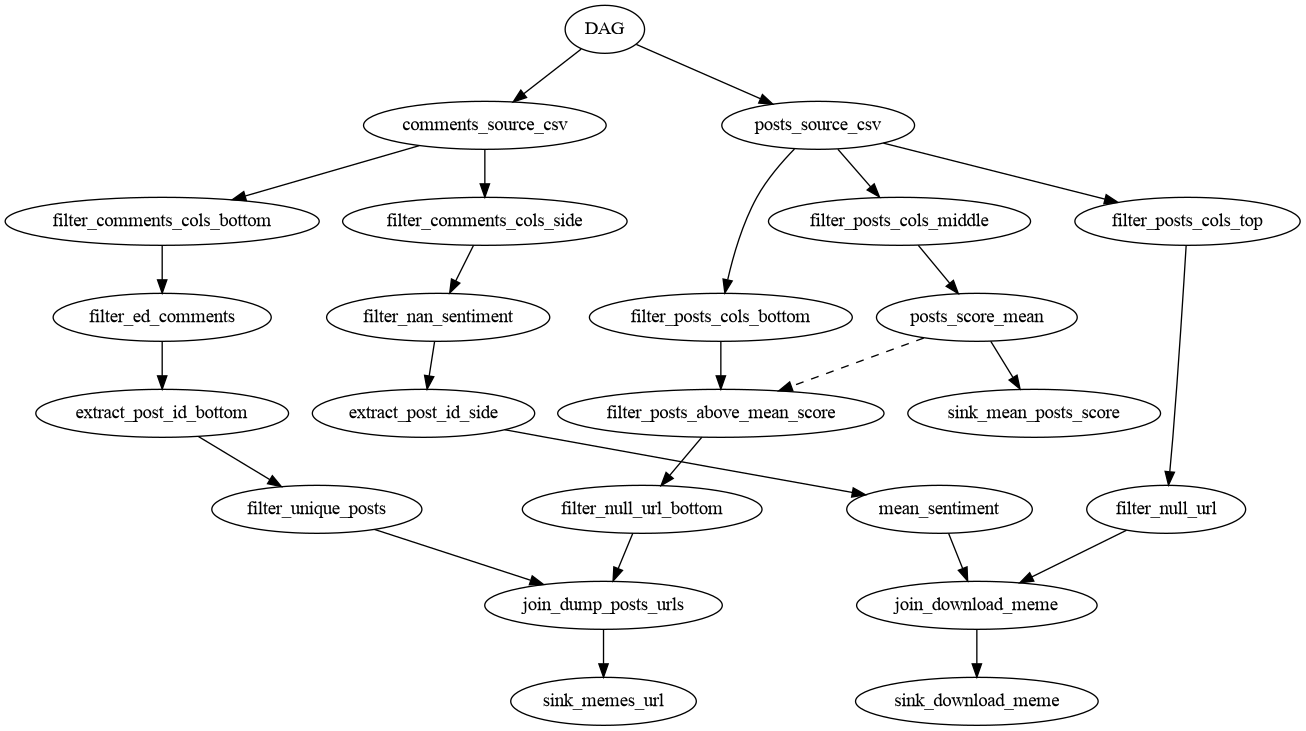
\includegraphics[width=\textwidth]{images/DAG.gv.png}
\caption{Render automático del DAG implementado.}
\end{figure}

Este grafo es generado con \texttt{graphviz} automáticamente al renderizar el DAG mediante \texttt{poetry run rma render-dag}. Los nodos con lineas punteadas indican que esa tarea está siendo paralelizada. Las aristas punteadas indican dependencias entre tareas.

Cada componente corre en su propio container de Docker. Necesita conocer las direcciones de las cuales sacar sus datos de entrada. Es por la complejidad asociada a generar este deploy que el presente TP incluye un módulo para definir DAGs y renderizar su \texttt{docker-compose.yaml} asociado.

Notar no todos los nodos que pueden ser paralelizados se implementaron de modo de hacerlo. Algunas simplificaciones con respecto al diseño se hicieron en base al esfuerzo requerido. Por ejemplo, los joins son paralelizables, pero recordemos que el DAG se diseño de modo tal que la cantidad de datos que les llega es la menor posible. O en el caso de \texttt{filter\_posts\_above\_mean\_score}, siendo el único nodo que recibe la salida de otro como dependencia, se evitó complicar la implementación paralelizándolo.

\section{Arquitectura}
\subsection{Diagrama de Secuencia}
\begin{figure}[H]
\centering
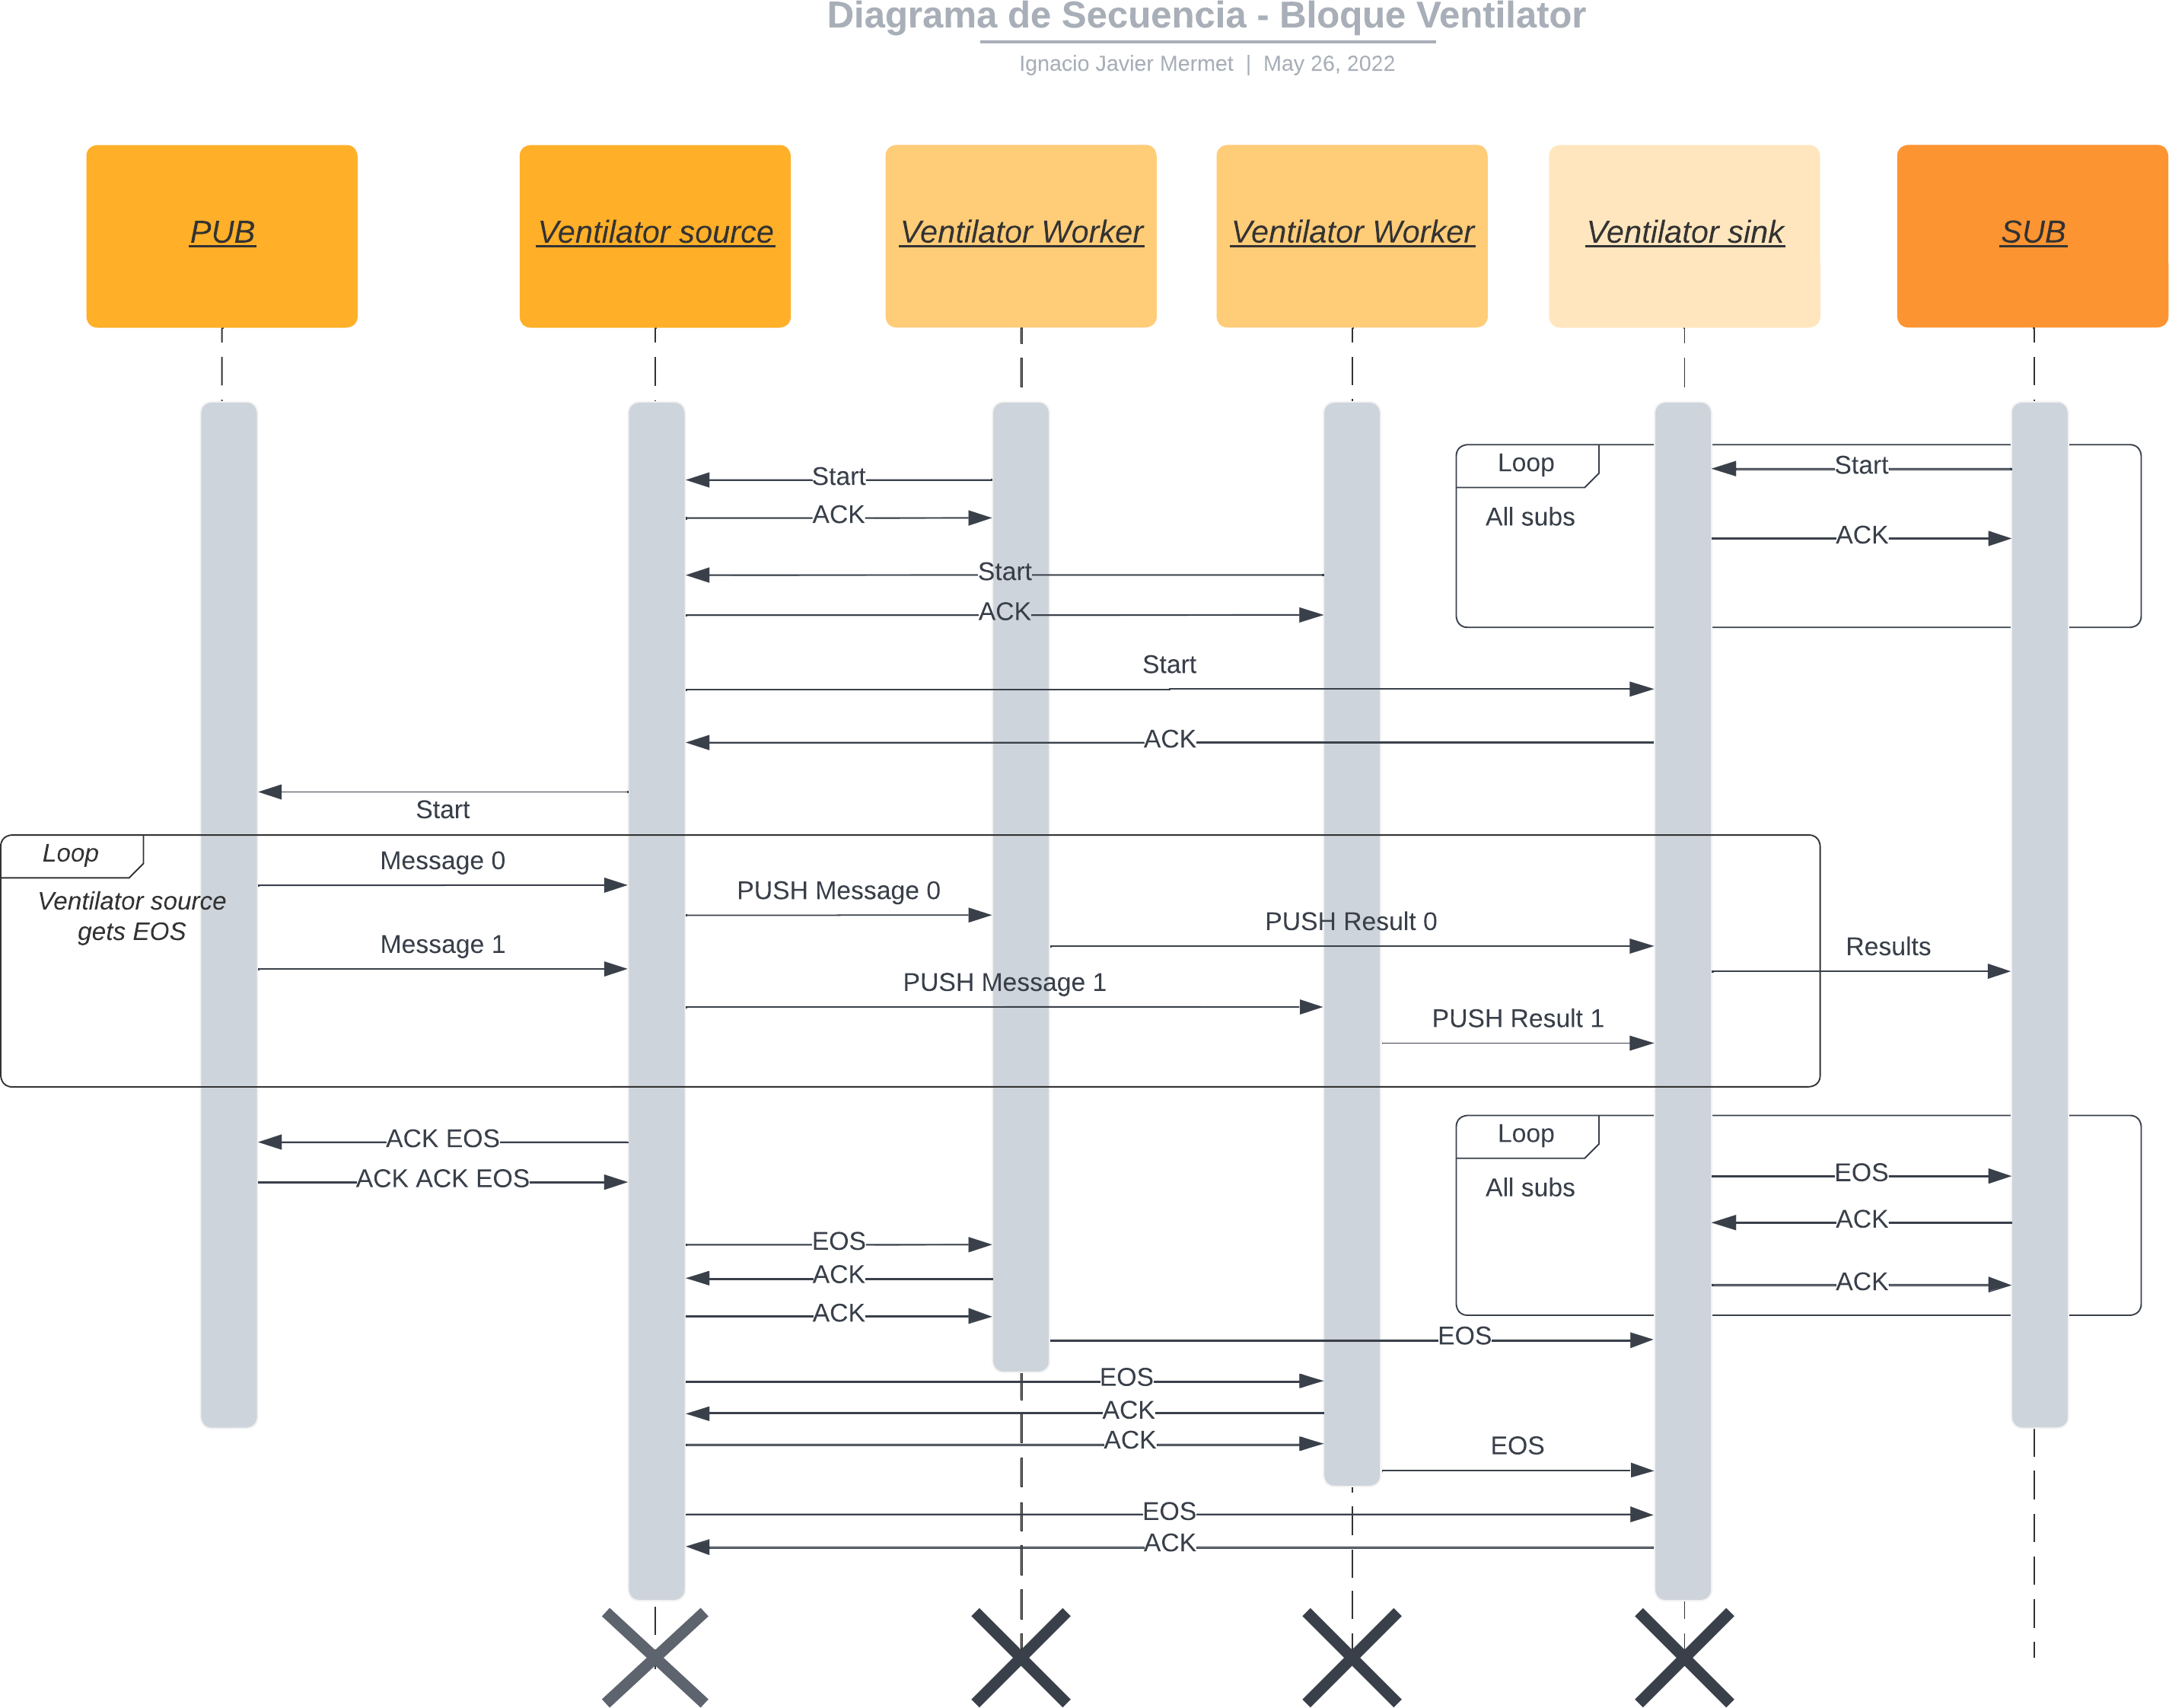
\includegraphics[width=\textwidth]{images/SequenceVentilator.png}
\caption{Diagrama de secuencia para bloques Ventilator.}
\end{figure}

\subsection{Diagrama de Robustez}
\begin{figure}[H]
\centering
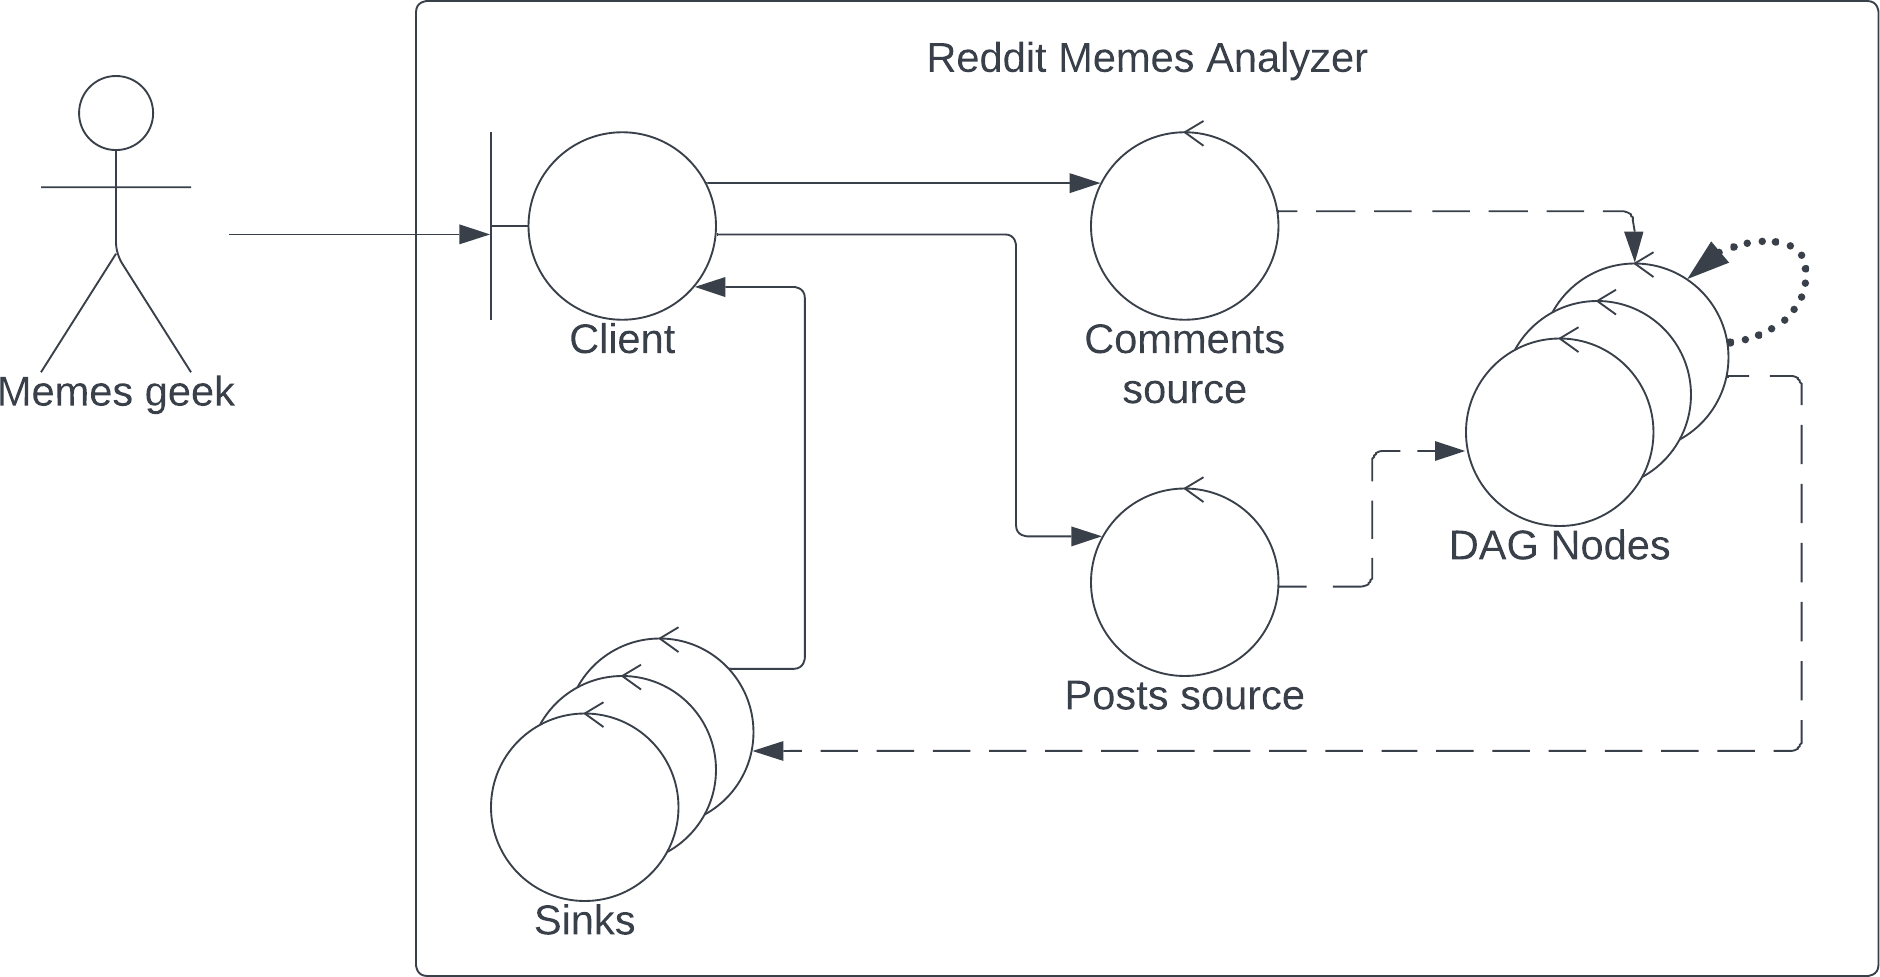
\includegraphics[width=\textwidth]{images/Robustez.png}
\caption{Diagrama de robustez.}
\end{figure}

\subsection{Diagrama de Despliegue}
\begin{figure}[H]
\centering
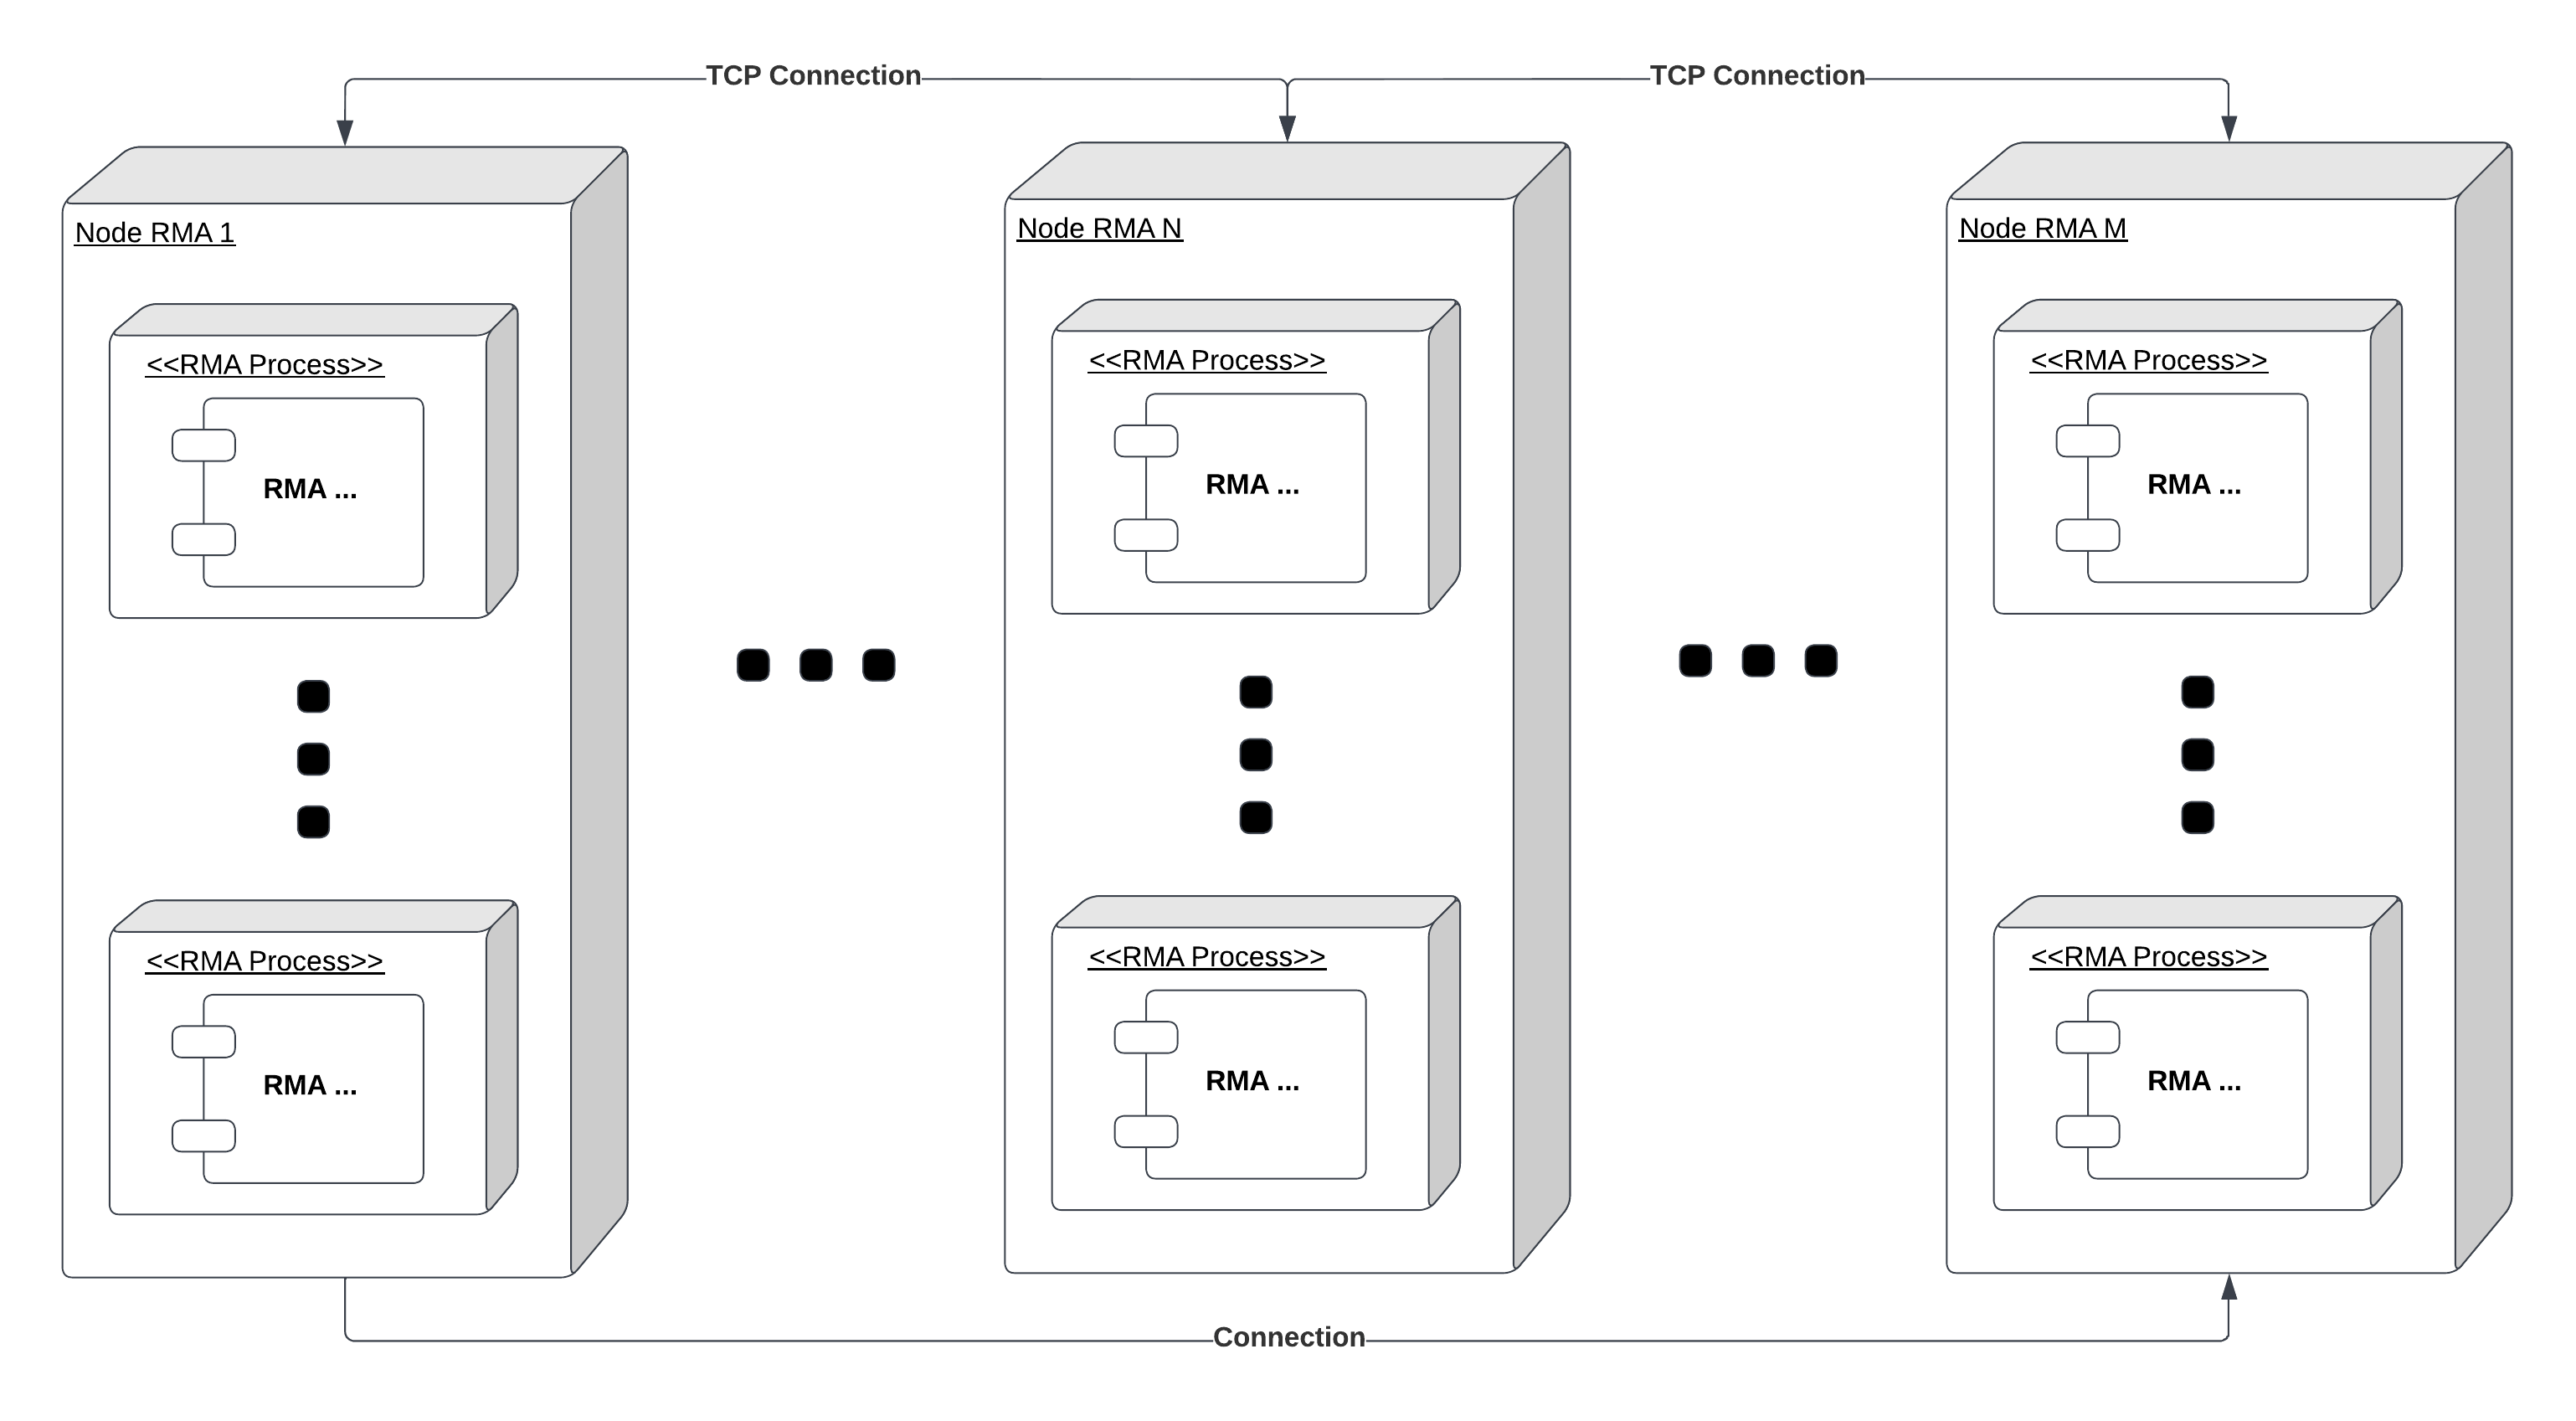
\includegraphics[width=\textwidth]{images/Despliegue.png}
\caption{Diagrama de despliegue del sistema.}
\end{figure}
Si bien sencillo, en este diagrama vemos que podemos tener $n$ nodos, cada nodo con $C_i$ containers ejecutando un entrypoint de \texttt{rma}. Mientras sean accesibles por red entre sí, cualquier configuración de nodos y containers por nodo será válida.

\subsection{Diagrama de Paquetes}
\begin{figure}[H]
\centering
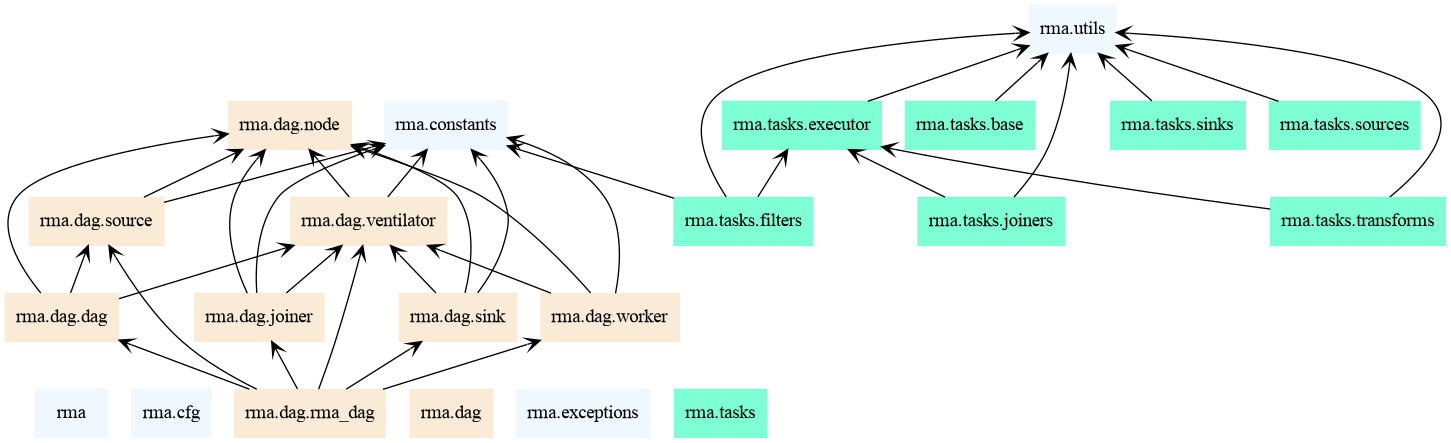
\includegraphics[width=\textwidth]{images/packages.png}
\caption{Diagrama de paquetes generado con \texttt{pyreverse}.}
\end{figure}

\section{Interfaz de los bloques del DAG}
De modo de poder interfeacear cómodamente los distintos nodos del DAG, se define una interfaz en común. Se usa \texttt{PUB/SUB} para entrada/salida de datos y \texttt{REQ/REP} para coordinar actividades.

Vemos en el siguiente diagrama los principales bloques del sistema:
\begin{itemize}
	\item Sources
	\item Sinks
	\item Ventilator Blocks: Bloques que paralelizan transformaciones o filtros
	\item Workers: Ejecutan transformaciones o filtros sin paralelismo
\end{itemize}

Los \texttt{Joins} cumplen con la misma interfaz y son muy cercanos a los \texttt{Workers} en comportamiento, con la salvedad de que reciben dos inputs.

\digraph{structs}{
    rankdir=TB;
    splines=polyline;
    node [shape=Mrecord];
    source [label="{Source | {<pub>PUB | <rep>REP}}"];
    ventilator_src [color=blue,label="{{<sub>SUB||<req_in>REQ}|{Ventilator|<req_out>REQ}|{<push>PUSH|<rep>REP}}"];
    ventilator_w1 [color=blue,label="{{<pull>PULL|<req>REQ}|Worker|<push>PUSH}"];
    ventilator_w2 [color=blue,label="{{<pull>PULL|<req>REQ}|Worker|<push>PUSH}"];
    ventilator_w3 [color=blue,label="{{<pull>PULL|<req>REQ}|Worker|<push>PUSH}"];
    ventilator_sink [color=blue,label="{{<pull>PULL|<rep_in>REP}|Sink|{<pub>PUB|<rep_out>REP}}"];
    worker [label="{{<sub>SUB|<req>REQ}|Worker|{<pub>PUB|<rep>REP}}"];
    sink [label="{{<sub>SUB|<req>REQ}|{Sink}}"];

    source:pub -> ventilator_src:sub;
    ventilator_src:req_in -> source:rep;

    ventilator_src:req_out -> ventilator_sink:rep_in;

    ventilator_src:push -> ventilator_w1:pull;
    ventilator_src:push -> ventilator_w2:pull;
    ventilator_src:push -> ventilator_w3:pull;

    ventilator_w1:req -> ventilator_src:rep;
    ventilator_w2:req -> ventilator_src:rep;
    ventilator_w3:req -> ventilator_src:rep;

    ventilator_w1:push -> ventilator_sink:pull;
    ventilator_w2:push -> ventilator_sink:pull;
    ventilator_w3:push -> ventilator_sink:pull;

    ventilator_sink:pub -> worker:sub;
    worker:req -> ventilator_sink:rep_out;

    worker:pub -> sink:sub;
    sink:req -> worker:rep;
}


\printbibliography

\end{document}
